\documentclass[aspectratio=169]{beamer}

% Theme and colors
\usetheme{Madrid}
\usecolortheme{whale}
\setbeamertemplate{navigation symbols}{}
\setbeamertemplate{footline}[frame number]

% Packages
\usepackage{listings}
\usepackage{xcolor}
\usepackage{tikz}
\usepackage{graphicx}
\usepackage{booktabs}

% Colors
\definecolor{javagreen}{rgb}{0.25,0.5,0.35}
\definecolor{javapurple}{rgb}{0.5,0,0.35}
\definecolor{javadocblue}{rgb}{0.25,0.35,0.75}
\definecolor{codebackground}{rgb}{0.95,0.95,0.95}

% Java code style
\lstdefinestyle{java}{
    language=Java,
    basicstyle=\ttfamily\scriptsize,
    keywordstyle=\color{javapurple}\bfseries,
    stringstyle=\color{javagreen},
    commentstyle=\color{javadocblue}\itshape,
    backgroundcolor=\color{codebackground},
    frame=single,
    framerule=0pt,
    showstringspaces=false,
    tabsize=2,
    breaklines=true,
    numbers=none
}

\lstset{style=java}

% Title information
\title[OOP: Inheritance \& Polymorphism]{Inheritance, Polymorphism, Abstract Classes \& Interfaces}
\subtitle{Object-Oriented Programming in Java}
\author{PT821: Object-Oriented Programming}
\institute{State University of Zanzibar (SUZA)}
\date{2025/2026 Academic Year}

\begin{document}

% Title slide
\begin{frame}
    \titlepage
\end{frame}

% Outline
\begin{frame}{Outline}
    \tableofcontents
\end{frame}

%===========================================
\section{Inheritance}
%===========================================

\begin{frame}{What is Inheritance?}
    \begin{block}{Definition}
        Inheritance is a mechanism where a new class \textbf{inherits} properties and behaviors from an existing class.
    \end{block}

    \vspace{0.5cm}

    \begin{columns}
        \begin{column}{0.5\textwidth}
            \textbf{Key Terms:}
            \begin{itemize}
                \item \textbf{Parent/Super Class} - The class being inherited from
                \item \textbf{Child/Sub Class} - The class that inherits
            \end{itemize}
        \end{column}
        \begin{column}{0.5\textwidth}
            \begin{center}
            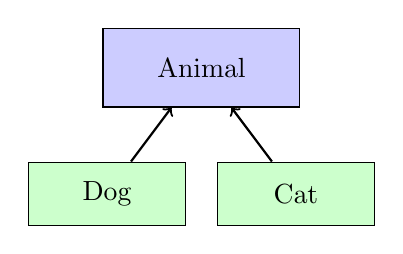
\begin{tikzpicture}[scale=0.8]
                \node[draw, rectangle, fill=blue!20, minimum width=2.5cm, minimum height=1cm] (parent) at (0,2) {Animal};
                \node[draw, rectangle, fill=green!20, minimum width=2cm, minimum height=0.8cm] (child1) at (-1.5,0) {Dog};
                \node[draw, rectangle, fill=green!20, minimum width=2cm, minimum height=0.8cm] (child2) at (1.5,0) {Cat};
                \draw[->, thick] (child1) -- (parent);
                \draw[->, thick] (child2) -- (parent);
            \end{tikzpicture}
            \end{center}
        \end{column}
    \end{columns}
\end{frame}

\begin{frame}{Why Use Inheritance?}
    \begin{columns}
        \begin{column}{0.5\textwidth}
            \textbf{Benefits:}
            \begin{enumerate}
                \item \textbf{Code Reusability} - Write once, use many times
                \item \textbf{Method Overriding} - Customize inherited behavior
                \item \textbf{Extensibility} - Easy to add new features
                \item \textbf{Maintainability} - Changes in one place
            \end{enumerate}
        \end{column}
        \begin{column}{0.5\textwidth}
            \begin{alertblock}{Real-World Analogy}
                A child inherits traits from parents but can have their own unique characteristics!
            \end{alertblock}
        \end{column}
    \end{columns}
\end{frame}

\begin{frame}[fragile]{The \texttt{extends} Keyword}
    \begin{block}{Syntax}
        \begin{lstlisting}
class ChildClass extends ParentClass {
    // Child class body
}
        \end{lstlisting}
    \end{block}

    \vspace{0.3cm}

    \textbf{Example:}
    \begin{lstlisting}
class Animal {
    String name;
    void eat() {
        System.out.println(name + " is eating");
    }
}

class Dog extends Animal {
    void bark() {
        System.out.println(name + " says Woof!");
    }
}
    \end{lstlisting}
\end{frame}

\begin{frame}{Types of Inheritance in Java}
    \begin{columns}
        \begin{column}{0.33\textwidth}
            \textbf{1. Single}
            \begin{center}
            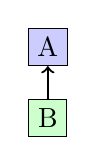
\begin{tikzpicture}[scale=0.6]
                \node[draw, rectangle, fill=blue!20] (a) at (0,1.5) {A};
                \node[draw, rectangle, fill=green!20] (b) at (0,0) {B};
                \draw[->, thick] (b) -- (a);
            \end{tikzpicture}
            \end{center}
            One parent, one child
        \end{column}
        \begin{column}{0.33\textwidth}
            \textbf{2. Multilevel}
            \begin{center}
            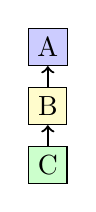
\begin{tikzpicture}[scale=0.6]
                \node[draw, rectangle, fill=blue!20] (a) at (0,2.5) {A};
                \node[draw, rectangle, fill=yellow!20] (b) at (0,1.25) {B};
                \node[draw, rectangle, fill=green!20] (c) at (0,0) {C};
                \draw[->, thick] (b) -- (a);
                \draw[->, thick] (c) -- (b);
            \end{tikzpicture}
            \end{center}
            Chain of inheritance
        \end{column}
        \begin{column}{0.33\textwidth}
            \textbf{3. Hierarchical}
            \begin{center}
            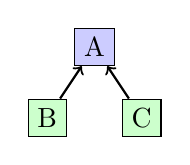
\begin{tikzpicture}[scale=0.6]
                \node[draw, rectangle, fill=blue!20] (a) at (0,1.5) {A};
                \node[draw, rectangle, fill=green!20] (b) at (-1,0) {B};
                \node[draw, rectangle, fill=green!20] (c) at (1,0) {C};
                \draw[->, thick] (b) -- (a);
                \draw[->, thick] (c) -- (a);
            \end{tikzpicture}
            \end{center}
            One parent, many children
        \end{column}
    \end{columns}

    \vspace{0.5cm}
    \begin{alertblock}{Note}
        Java does NOT support multiple inheritance with classes (use interfaces instead).
    \end{alertblock}
\end{frame}

\begin{frame}[fragile]{The \texttt{super} Keyword}
    The \texttt{super} keyword refers to the parent class.

    \vspace{0.3cm}

    \textbf{Three Uses:}

    \begin{columns}
        \begin{column}{0.5\textwidth}
            \textbf{1. Call Parent Constructor}
            \begin{lstlisting}
class Dog extends Animal {
    Dog(String name) {
        super(name); // calls Animal()
    }
}
            \end{lstlisting}
        \end{column}
        \begin{column}{0.5\textwidth}
            \textbf{2. Access Parent Method}
            \begin{lstlisting}
void display() {
    super.display(); // parent's
    // then child's code
}
            \end{lstlisting}
        \end{column}
    \end{columns}

    \vspace{0.3cm}

    \textbf{3. Access Parent Variable:} \texttt{super.variableName}
\end{frame}

\begin{frame}[fragile]{Complete Inheritance Example}
    \begin{lstlisting}
class Person {
    String name;
    int age;

    Person(String name, int age) {
        this.name = name;
        this.age = age;
    }

    void introduce() {
        System.out.println("I am " + name + ", " + age + " years old");
    }
}

class Student extends Person {
    String studentId;

    Student(String name, int age, String studentId) {
        super(name, age);  // Call parent constructor
        this.studentId = studentId;
    }

    void study() {
        System.out.println(name + " is studying");
    }
}
    \end{lstlisting}
\end{frame}

%===========================================
\section{Polymorphism}
%===========================================

\begin{frame}{What is Polymorphism?}
    \begin{block}{Definition}
        \textbf{Polymorphism} = "many forms" - the ability of an object to take different forms.
    \end{block}

    \vspace{0.5cm}

    \begin{columns}
        \begin{column}{0.5\textwidth}
            \textbf{Two Types:}
            \begin{enumerate}
                \item \textbf{Compile-time} (Static)
                    \begin{itemize}
                        \item Method Overloading
                    \end{itemize}
                \item \textbf{Runtime} (Dynamic)
                    \begin{itemize}
                        \item Method Overriding
                    \end{itemize}
            \end{enumerate}
        \end{column}
        \begin{column}{0.5\textwidth}
            \begin{exampleblock}{Real-World Example}
                A person can be a student, employee, and parent - same person, different roles!
            \end{exampleblock}
        \end{column}
    \end{columns}
\end{frame}

\begin{frame}[fragile]{Method Overloading (Compile-time)}
    \textbf{Same method name, different parameters}

    \begin{lstlisting}
class Calculator {
    // Two integers
    int add(int a, int b) {
        return a + b;
    }

    // Three integers
    int add(int a, int b, int c) {
        return a + b + c;
    }

    // Two doubles
    double add(double a, double b) {
        return a + b;
    }
}
    \end{lstlisting}

    \begin{alertblock}{Rules}
        Must differ in: number of parameters, type of parameters, or order of parameters.
    \end{alertblock}
\end{frame}

\begin{frame}[fragile]{Method Overriding (Runtime)}
    \textbf{Child class provides specific implementation of parent's method}

    \begin{lstlisting}
class Animal {
    void makeSound() {
        System.out.println("Some sound");
    }
}

class Dog extends Animal {
    @Override
    void makeSound() {
        System.out.println("Woof! Woof!");
    }
}

class Cat extends Animal {
    @Override
    void makeSound() {
        System.out.println("Meow!");
    }
}
    \end{lstlisting}

    \begin{block}{@Override Annotation}
        Tells compiler we intend to override - catches errors!
    \end{block}
\end{frame}

\begin{frame}[fragile]{Polymorphism in Action}
    \begin{lstlisting}
public class Main {
    public static void main(String[] args) {
        // Parent reference, child objects
        Animal myAnimal;

        myAnimal = new Dog();
        myAnimal.makeSound();  // Output: Woof! Woof!

        myAnimal = new Cat();
        myAnimal.makeSound();  // Output: Meow!

        // Array of Animals
        Animal[] animals = {new Dog(), new Cat(), new Dog()};
        for (Animal a : animals) {
            a.makeSound();  // Each calls its own version!
        }
    }
}
    \end{lstlisting}

    \begin{exampleblock}{Key Point}
        The same method call produces different results based on the actual object type!
    \end{exampleblock}
\end{frame}

\begin{frame}{Overloading vs Overriding}
    \begin{table}
        \small
        \begin{tabular}{p{4cm}|p{4cm}|p{4cm}}
            \toprule
            \textbf{Aspect} & \textbf{Overloading} & \textbf{Overriding} \\
            \midrule
            When decided & Compile-time & Runtime \\
            \hline
            Where & Same class & Parent-Child \\
            \hline
            Parameters & Must differ & Must be same \\
            \hline
            Return type & Can differ & Must be same/covariant \\
            \hline
            Keyword & None & @Override \\
            \bottomrule
        \end{tabular}
    \end{table}
\end{frame}

%===========================================
\section{Abstract Classes}
%===========================================

\begin{frame}{What is an Abstract Class?}
    \begin{block}{Definition}
        An \textbf{abstract class} is a class that cannot be instantiated and may contain abstract methods (methods without implementation).
    \end{block}

    \vspace{0.5cm}

    \textbf{Key Characteristics:}
    \begin{itemize}
        \item Declared with \texttt{abstract} keyword
        \item \textbf{Cannot} create objects directly
        \item \textbf{Can} have both abstract and concrete methods
        \item \textbf{Can} have constructors and instance variables
        \item Child classes \textbf{must} implement all abstract methods
    \end{itemize}

    \begin{alertblock}{Purpose}
        Provides a common base with some implementation, forcing subclasses to complete the rest.
    \end{alertblock}
\end{frame}

\begin{frame}[fragile]{Abstract Class Syntax}
    \begin{lstlisting}
abstract class Shape {
    String color;

    // Constructor
    Shape(String color) {
        this.color = color;
    }

    // Abstract method - no body!
    abstract double calculateArea();

    // Concrete method - has body
    void displayColor() {
        System.out.println("Color: " + color);
    }
}
    \end{lstlisting}

    \begin{block}{Note}
        Abstract methods end with semicolon - no curly braces!
    \end{block}
\end{frame}

\begin{frame}[fragile]{Implementing Abstract Class}
    \begin{lstlisting}
class Circle extends Shape {
    double radius;

    Circle(String color, double radius) {
        super(color);
        this.radius = radius;
    }

    @Override
    double calculateArea() {
        return Math.PI * radius * radius;
    }
}

class Rectangle extends Shape {
    double width, height;

    Rectangle(String color, double w, double h) {
        super(color);
        this.width = w;
        this.height = h;
    }

    @Override
    double calculateArea() {
        return width * height;
    }
}
    \end{lstlisting}
\end{frame}

\begin{frame}[fragile]{Using Abstract Classes}
    \begin{lstlisting}
public class Main {
    public static void main(String[] args) {
        // Shape s = new Shape("Red");  // ERROR! Cannot instantiate

        Shape circle = new Circle("Red", 5.0);
        Shape rect = new Rectangle("Blue", 4.0, 6.0);

        System.out.println("Circle area: " + circle.calculateArea());
        System.out.println("Rectangle area: " + rect.calculateArea());

        circle.displayColor();  // Inherited concrete method
    }
}
    \end{lstlisting}

    \textbf{Output:}
    \begin{verbatim}
Circle area: 78.54
Rectangle area: 24.0
Color: Red
    \end{verbatim}
\end{frame}

%===========================================
\section{Interfaces}
%===========================================

\begin{frame}{What is an Interface?}
    \begin{block}{Definition}
        An \textbf{interface} is a contract that defines what a class must do, but not how it does it.
    \end{block}

    \vspace{0.5cm}

    \textbf{Key Characteristics:}
    \begin{itemize}
        \item All methods are \textbf{public abstract} by default
        \item All variables are \textbf{public static final} (constants)
        \item A class \textbf{implements} an interface
        \item A class can implement \textbf{multiple} interfaces
        \item Cannot have constructors
    \end{itemize}

    \begin{exampleblock}{Real-World Analogy}
        Like a contract or job description - it says what must be done, but not how to do it.
    \end{exampleblock}
\end{frame}

\begin{frame}[fragile]{Interface Syntax}
    \begin{lstlisting}
interface Drawable {
    void draw();  // public abstract by default
}

interface Resizable {
    void resize(double factor);
    double getSize();
}

// Implementing interfaces
class Circle implements Drawable, Resizable {
    double radius = 5.0;

    @Override
    public void draw() {
        System.out.println("Drawing circle with radius " + radius);
    }

    @Override
    public void resize(double factor) {
        radius *= factor;
    }

    @Override
    public double getSize() {
        return radius;
    }
}
    \end{lstlisting}
\end{frame}

\begin{frame}[fragile]{Multiple Interface Implementation}
    \begin{center}
    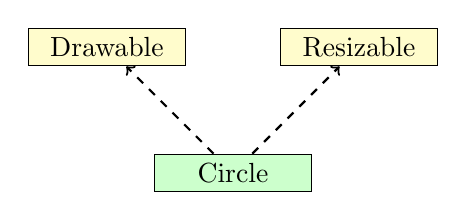
\begin{tikzpicture}[scale=0.8]
        \node[draw, rectangle, fill=yellow!20, minimum width=2cm] (d) at (-2,2) {Drawable};
        \node[draw, rectangle, fill=yellow!20, minimum width=2cm] (r) at (2,2) {Resizable};
        \node[draw, rectangle, fill=green!20, minimum width=2cm] (c) at (0,0) {Circle};
        \draw[->, thick, dashed] (c) -- (d);
        \draw[->, thick, dashed] (c) -- (r);
    \end{tikzpicture}
    \end{center}

    \begin{lstlisting}
class Circle implements Drawable, Resizable {
    // Must implement ALL methods from BOTH interfaces
}
    \end{lstlisting}

    \begin{alertblock}{This is how Java achieves "multiple inheritance"}
        A class can extend only ONE class but implement MANY interfaces!
    \end{alertblock}
\end{frame}

\begin{frame}{Abstract Class vs Interface}
    \begin{table}
        \small
        \begin{tabular}{p{4cm}|p{4cm}|p{4cm}}
            \toprule
            \textbf{Feature} & \textbf{Abstract Class} & \textbf{Interface} \\
            \midrule
            Methods & Abstract + Concrete & Abstract only* \\
            \hline
            Variables & Any type & Constants only \\
            \hline
            Constructor & Yes & No \\
            \hline
            Inheritance & extends (single) & implements (multiple) \\
            \hline
            Access modifiers & Any & Public only \\
            \hline
            Use when & IS-A relationship & CAN-DO capability \\
            \bottomrule
        \end{tabular}
    \end{table}

    \vspace{0.3cm}
    \small *Java 8+ allows default and static methods in interfaces
\end{frame}

\begin{frame}{When to Use What?}
    \begin{columns}
        \begin{column}{0.5\textwidth}
            \textbf{Use Abstract Class when:}
            \begin{itemize}
                \item Classes share common code
                \item Need non-public members
                \item Need constructors
                \item Want to provide default behavior
            \end{itemize}

            \vspace{0.3cm}
            \textbf{Example:} Animal $\rightarrow$ Dog, Cat
        \end{column}
        \begin{column}{0.5\textwidth}
            \textbf{Use Interface when:}
            \begin{itemize}
                \item Unrelated classes need same behavior
                \item Need multiple inheritance
                \item Define a contract/capability
                \item Want loose coupling
            \end{itemize}

            \vspace{0.3cm}
            \textbf{Example:} Comparable, Serializable
        \end{column}
    \end{columns}
\end{frame}

%===========================================
\section{Combining All Concepts}
%===========================================

\begin{frame}[fragile]{Real-World Example: Payment System}
    \begin{lstlisting}
// Interface - defines capability
interface Payable {
    void processPayment(double amount);
}

// Abstract class - common base
abstract class Payment implements Payable {
    protected String transactionId;

    Payment() {
        this.transactionId = generateId();
    }

    private String generateId() {
        return "TXN" + System.currentTimeMillis();
    }

    abstract void validate();  // Each payment validates differently
}
    \end{lstlisting}
\end{frame}

\begin{frame}[fragile]{Payment System (Continued)}
    \begin{lstlisting}
class CreditCard extends Payment {
    private String cardNumber;

    CreditCard(String cardNumber) {
        super();
        this.cardNumber = cardNumber;
    }

    @Override
    void validate() {
        System.out.println("Validating card: " + cardNumber);
    }

    @Override
    public void processPayment(double amount) {
        validate();
        System.out.println("Processing $" + amount + " via Credit Card");
    }
}

class MobileMoney extends Payment {
    private String phoneNumber;
    // Similar implementation...
}
    \end{lstlisting}
\end{frame}

\begin{frame}[fragile]{Using the Payment System}
    \begin{lstlisting}
public class PaymentDemo {
    public static void main(String[] args) {
        // Polymorphism - same interface, different implementations
        Payable[] payments = {
            new CreditCard("1234-5678-9012-3456"),
            new MobileMoney("+255-123-456-789"),
            new BankTransfer("SUZA-ACCOUNT-001")
        };

        double amount = 50000.0;

        for (Payable payment : payments) {
            payment.processPayment(amount);
            System.out.println("---");
        }
    }
}
    \end{lstlisting}

    \begin{exampleblock}{Key Benefit}
        Easy to add new payment methods without changing existing code!
    \end{exampleblock}
\end{frame}

%===========================================
\section{Summary}
%===========================================

\begin{frame}{Key Takeaways}
    \begin{columns}
        \begin{column}{0.5\textwidth}
            \textbf{Inheritance}
            \begin{itemize}
                \item Code reuse via \texttt{extends}
                \item \texttt{super} for parent access
                \item Single inheritance only
            \end{itemize}

            \vspace{0.3cm}

            \textbf{Polymorphism}
            \begin{itemize}
                \item Overloading = same name, different params
                \item Overriding = new implementation
                \item Runtime flexibility
            \end{itemize}
        \end{column}
        \begin{column}{0.5\textwidth}
            \textbf{Abstract Classes}
            \begin{itemize}
                \item Cannot instantiate
                \item Mix of abstract + concrete
                \item For IS-A relationships
            \end{itemize}

            \vspace{0.3cm}

            \textbf{Interfaces}
            \begin{itemize}
                \item Pure contract
                \item Multiple implementation
                \item For CAN-DO capabilities
            \end{itemize}
        \end{column}
    \end{columns}
\end{frame}

\begin{frame}{Best Practices}
    \begin{enumerate}
        \item \textbf{Favor composition over inheritance} when possible
        \item \textbf{Program to interfaces}, not implementations
        \item \textbf{Use @Override} annotation always
        \item \textbf{Keep inheritance hierarchies shallow} (max 3-4 levels)
        \item \textbf{Don't use inheritance} just for code reuse
        \item \textbf{Abstract classes} for related classes with shared code
        \item \textbf{Interfaces} for unrelated classes with common behavior
    \end{enumerate}
\end{frame}

\begin{frame}{Practice Exercises}
    \begin{enumerate}
        \item Create a \textbf{Vehicle} hierarchy with Car, Motorcycle, Bicycle
        \item Implement a \textbf{Shape} system with Circle, Rectangle, Triangle
        \item Design a \textbf{Bank Account} system with Savings, Checking accounts
        \item Create an \textbf{E-commerce} product system with Books, Electronics
        \item Implement a \textbf{Zoo} management system with different animals
    \end{enumerate}

    \vspace{0.5cm}

    \begin{alertblock}{Challenge}
        For each exercise, use a combination of inheritance, abstract classes, and interfaces!
    \end{alertblock}
\end{frame}

\begin{frame}
    \begin{center}
        \Huge Thank You!

        \vspace{1cm}

        \Large Questions?

        \vspace{1cm}

        \normalsize
        PT821: Object-Oriented Programming\\
        State University of Zanzibar (SUZA)
    \end{center}
\end{frame}

\end{document}
